\section{Ignitions}
\pgfdeclareimage[width=1.0\paperwidth]{header-image}{header_images/red_lightn}

\begin{frame}<1-3>
    \frametitle{Igntions}
    \framesubtitle{Humans and Natural < Humans + Natural}

	\begin{textblock*}{12cm}(0cm,1.5cm)
    \begin{tikzpicture}
        \node[anchor=south west,inner sep=0] (image) at (0,0) {
            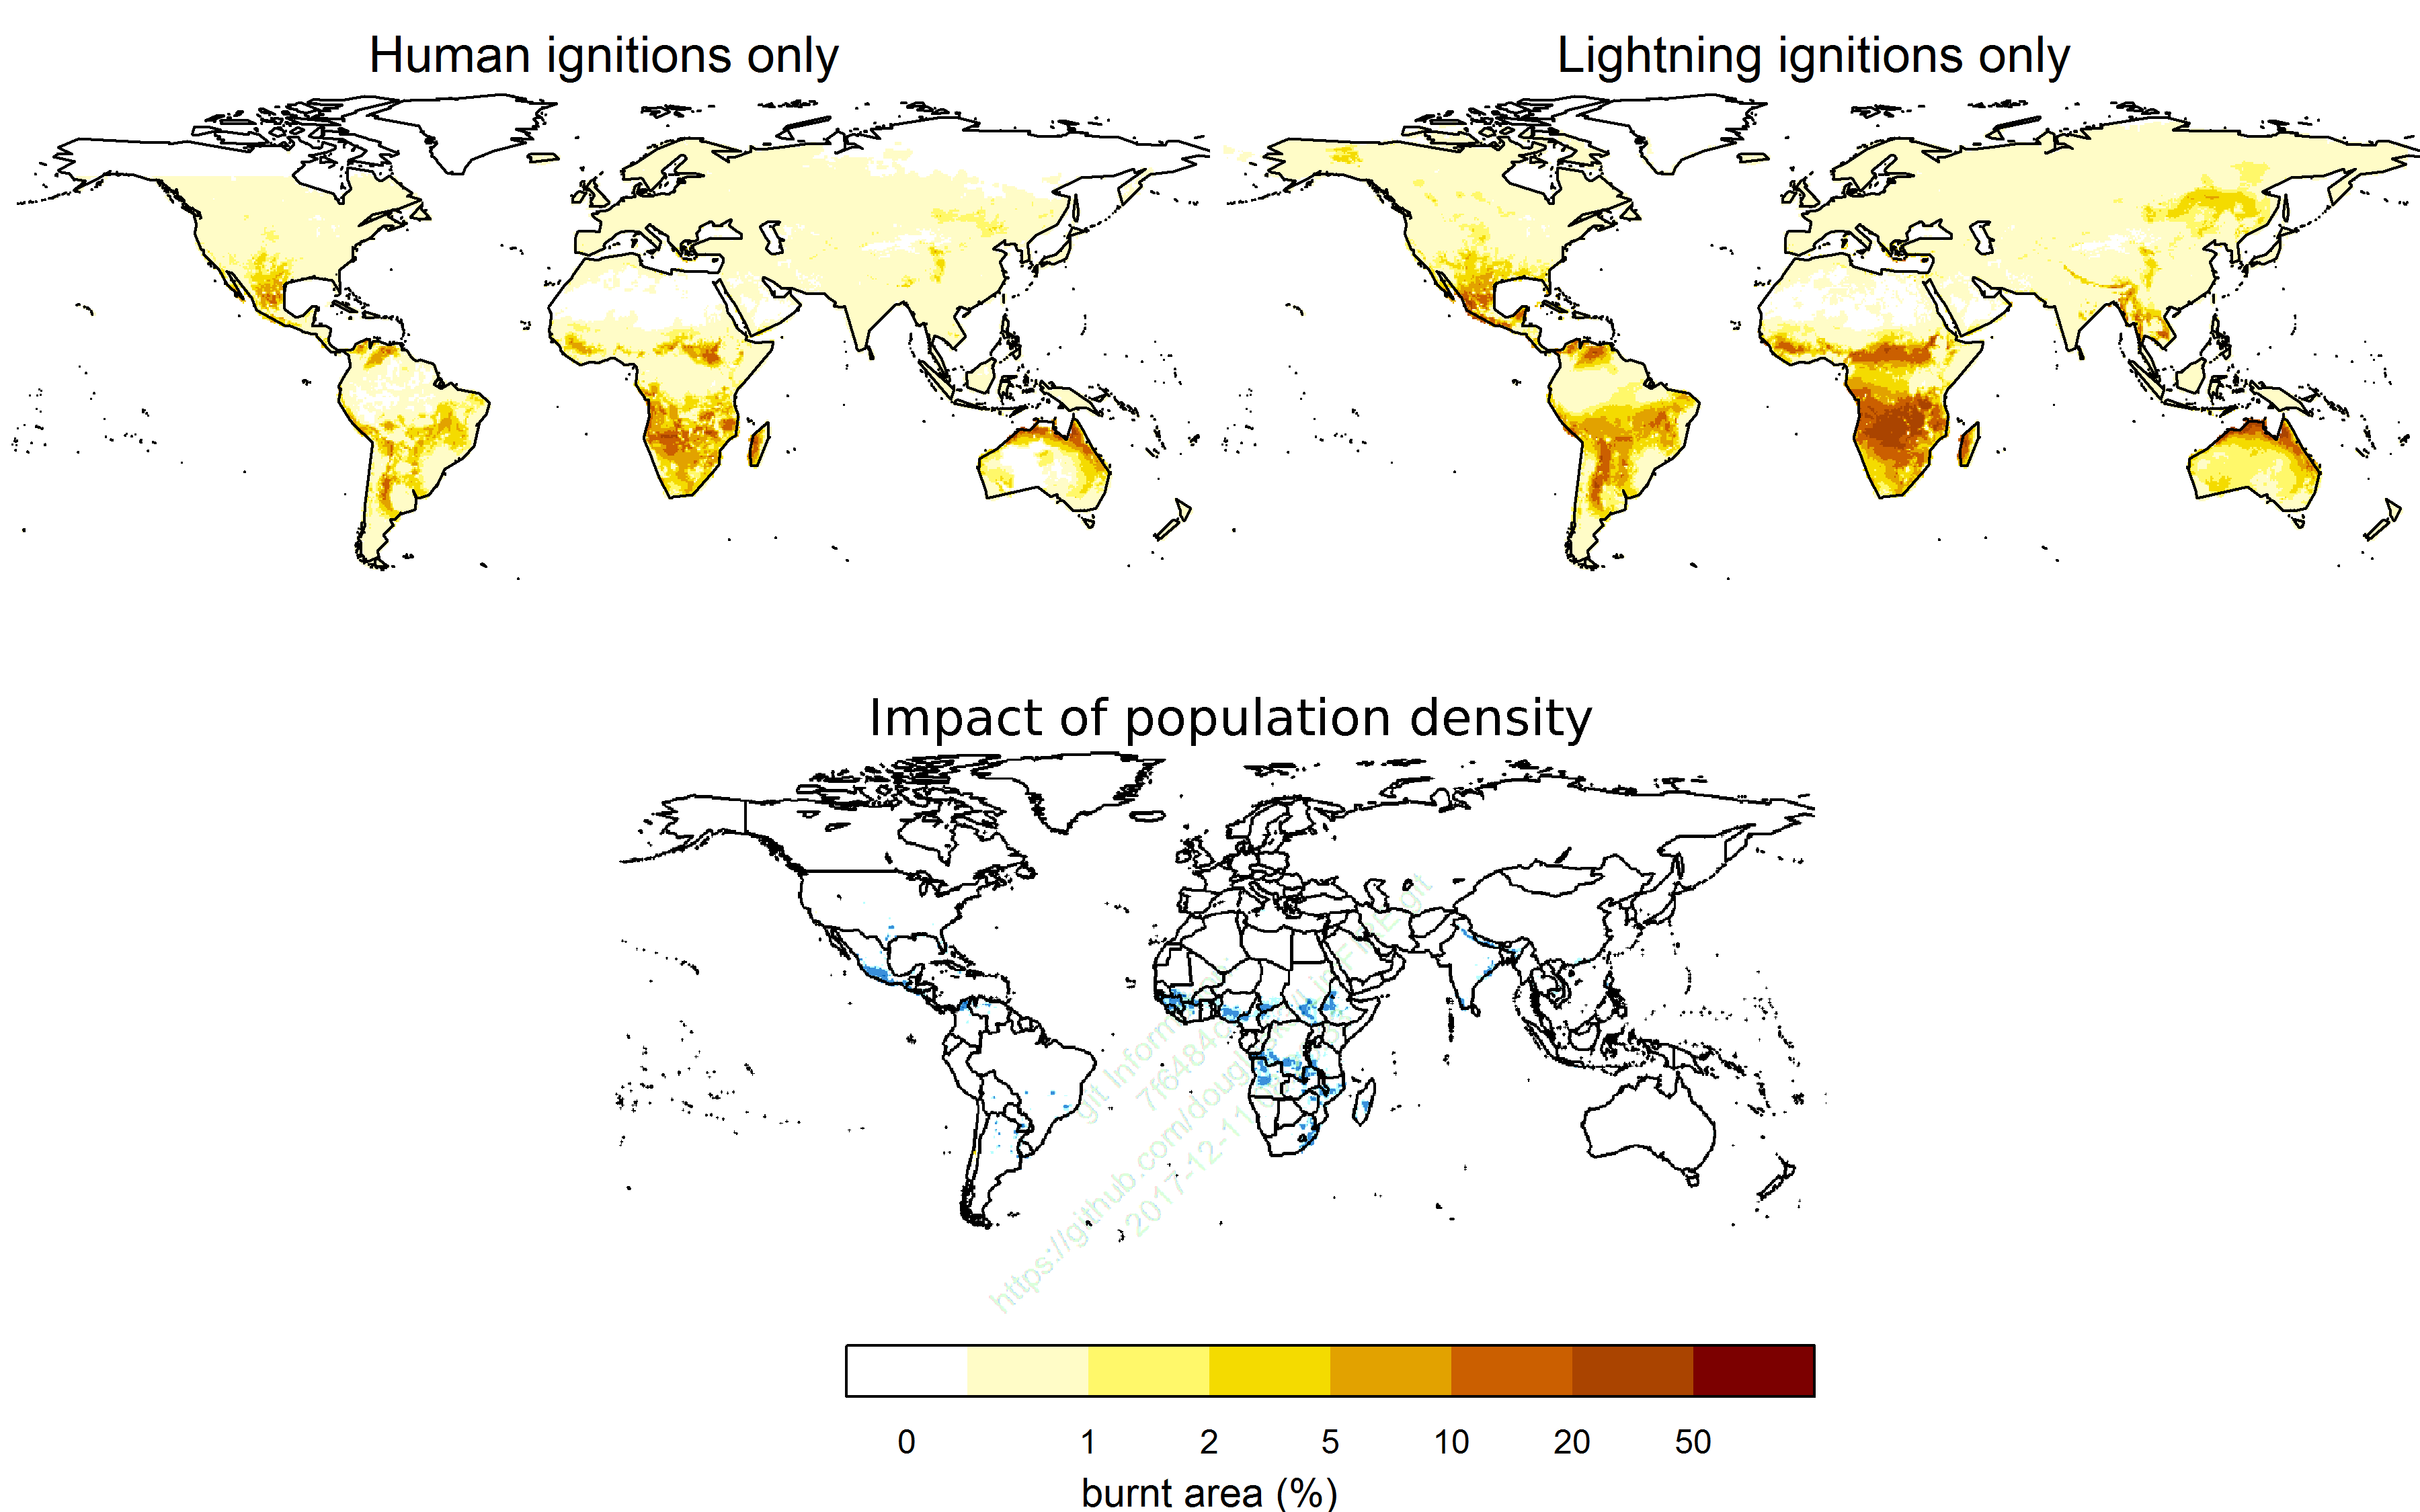
\includegraphics[width=12.0cm]{images/igntitions/IgntionInfoSourceAdding}
        };

        \visible<-1> {\draw[white, fill = white] (6.0,4.4) -- (12.0,4.4) -- (12.0,7.4) -- (6.0,7.4) -- (6.0,4.4);}
        \visible<-2> {\draw[white, fill = white] (0.0,1.0) -- (12.0,1.0) -- (12.0,4.5) -- (0.0,4.5) -- (0.0,1.0);}
    \end{tikzpicture}
	\end{textblock*}
\end{frame}


